\section{Linear Quadratic Regulator} \label{sec:lqr}
The first design approach for the inner controller is a state feedback. The compensator gain is obtained using a Linear Quadratic Regulator (LQR). First, a state space model of the system is created based on the equations derived in \autoref{chap:model}. Then, a cost function based on the state errors and the input usage is minimized in order to calculate the controller gains. 

\subsection{State Space Model}
The linearized model derived in \autoref{sec:linearizationModel}, consisting of \autoref{eq:x_pos_model_lin} to \ref{eq:psi_model_lin}, needs to be represented in state space form in order to design a state space controller. In order to do that, the 3 degree of freedom model used for the control of the vessel is represented as
\begin{flalign}
    \vec{\dot{x}}(t) &= \vec{A} \vec{x}(t) + \vec{B} \vec{u}(t)
    \label{xDotLinear} \\
    \vec{y}(t) &= \vec{C} \vec{x}(t) + \vec{D} \vec{u}(t)
    \label{yLinear} 
\end{flalign}
\begin{where}
    \va{\vec{x}}{is the state vector}{}
    \va{\vec{u}}{is the input vector}{}
    \va{\vec{y}}{is the output vector}{}
    \va{\vec{A}}{is the state matrix}{}
    \va{\vec{B}}{is the input matrix}{}
    \va{\vec{C}}{is the output matrix}{}
    \va{\vec{D}}{is the feed-forward matrix}{}
\end{where}

The state vector is constituted by the angle and velocity in yaw as well as the velocity in x in the body frame. The outputs of the system are yaw angle and velocity in x in the body frame. The input to the system is composed of the two forces applied in the body frame.
%It is important to notice that the position of the vessel in the body reference frame represents the  integration of the velocity along the body frame directions.
%This can also be seen as the position of the vessel with respect to a frame whose origin coincides with that of the NED frame and whose orientation coincides with that of the body frame \cite[p. 173]{TFossen}. 

\begin{minipage}{0.32\linewidth}
    \begin{flalign}
        \vec{x(t)} = 
        \begin{bmatrix}
            \psi\\
            \dot{\psi}\\
            \dot{x}_{b} \\
        \end{bmatrix} \nonumber
        \label{xVector}
    \end{flalign}  
\end{minipage}\hfill
%\hspace{0.03\linewidth}
\begin{minipage}{0.32\linewidth}
    \begin{flalign}
        \vec{y(t)} = 
        \begin{bmatrix}
            \phi \\
            \dot{x}_{b} \\
        \end{bmatrix} \nonumber
        \label{yVector}
    \end{flalign}
\end{minipage}\hfill
%\hspace{0.03\linewidth}
\begin{minipage}{0.32\linewidth}
    \begin{flalign}
        \vec{u(t)}= 
        \begin{bmatrix}
            F_1 \\
            F_2 
        \end{bmatrix}
        \label{uVector}
    \end{flalign} \nonumber
\end{minipage}\hfill

The resulting $\vec{A}$, $\vec{B}$, $\vec{C}$ and $\vec{D}$ matrices are
\begin{flalign}
    \vec{A} &=
    \begin{bmatrix}
        \ 0 & 1                   & 0                \ \ \ \\ 
        \ 0 & -\frac{d_\psi}{I_z} & 0                \ \ \ \\ 
        \ 0 & 0                   & -\frac{d_x}{m_x} \ \ \     
    \end{bmatrix}\rule{30px}{0px}
    \vec{B} = 
    \begin{bmatrix}
        \ 0               & 0                \ \ \ \\
        \ \frac{l_1}{I_z} & -\frac{l_2}{I_z} \ \ \ \\   
        \ \frac{1}{m_x}   & \frac{1}{m_x}    \ \ \
    \end{bmatrix}\rule{30px}{0px}
    \vec{C} =   
    \begin{bmatrix}
        \ 1 & 0 & 0  \ \ \ \\ 
        \ 0 & 0 & 1  \ \ \    
    \end{bmatrix}
    \label{eqStateSpaceABC}
\end{flalign}
and the $\vec{D}$ matrix is zero.

\subsection{Controller Design}
As the controller eventually must be implemented the design is carried out in the discrete domain. To do so, it is necessary to discretize the system. A discrete state space model can be expressed as,
%
\begin{flalign}
  \vec{x}(k+1) &= \vec{A_z} \vec{x}(k) + \vec{B_z} \vec{u}(k)
  \label{xDotLinearDiscrete} \\
  \vec{y}(k)   &= \vec{C_z} \vec{x}(k) + \vec{D_z} \vec{u}(k) \ \ ,
  \label{yLinearDiscrete} 
\end{flalign}
%
where the z subindexes indicate the matrices being in the discrete domain and k is the sample index. The model is discretized using zero order hold, with a sampling time, $T_s = 0.05 \mathrm{s}$. This sampling time is suitable as it is faster than the system's dynamics, which ensures the controller will be able to react faster to changes in the system. In \autoref{fig:discreteSSBlock} the discrete system is shown in a block diagram. The feed forward matrix is excluded as it is not present in this system.
%
\begin{figure}[H]
  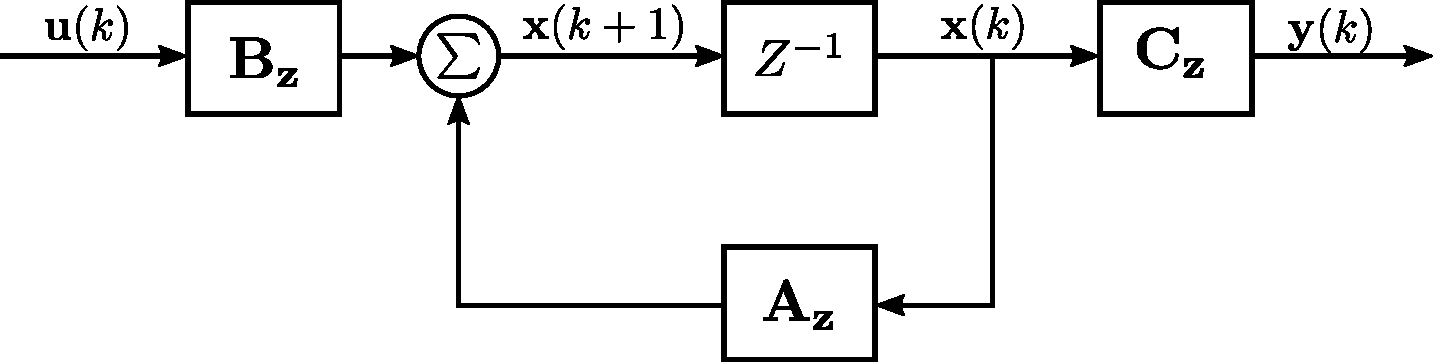
\includegraphics[width=0.6\textwidth]{figures/discreteSystemBlockDiagram}
  \caption{Block diagram of the discrete system without feed forward.}
  \label{fig:discreteSSBlock}
\end{figure}
%
In order to track a reference and handle input disturbances, it is chosen to also include an integral controller in the design. The final control structure is seen in \autoref{fig:blockConrolDesignLQR}.
%
\begin{figure}[H]
  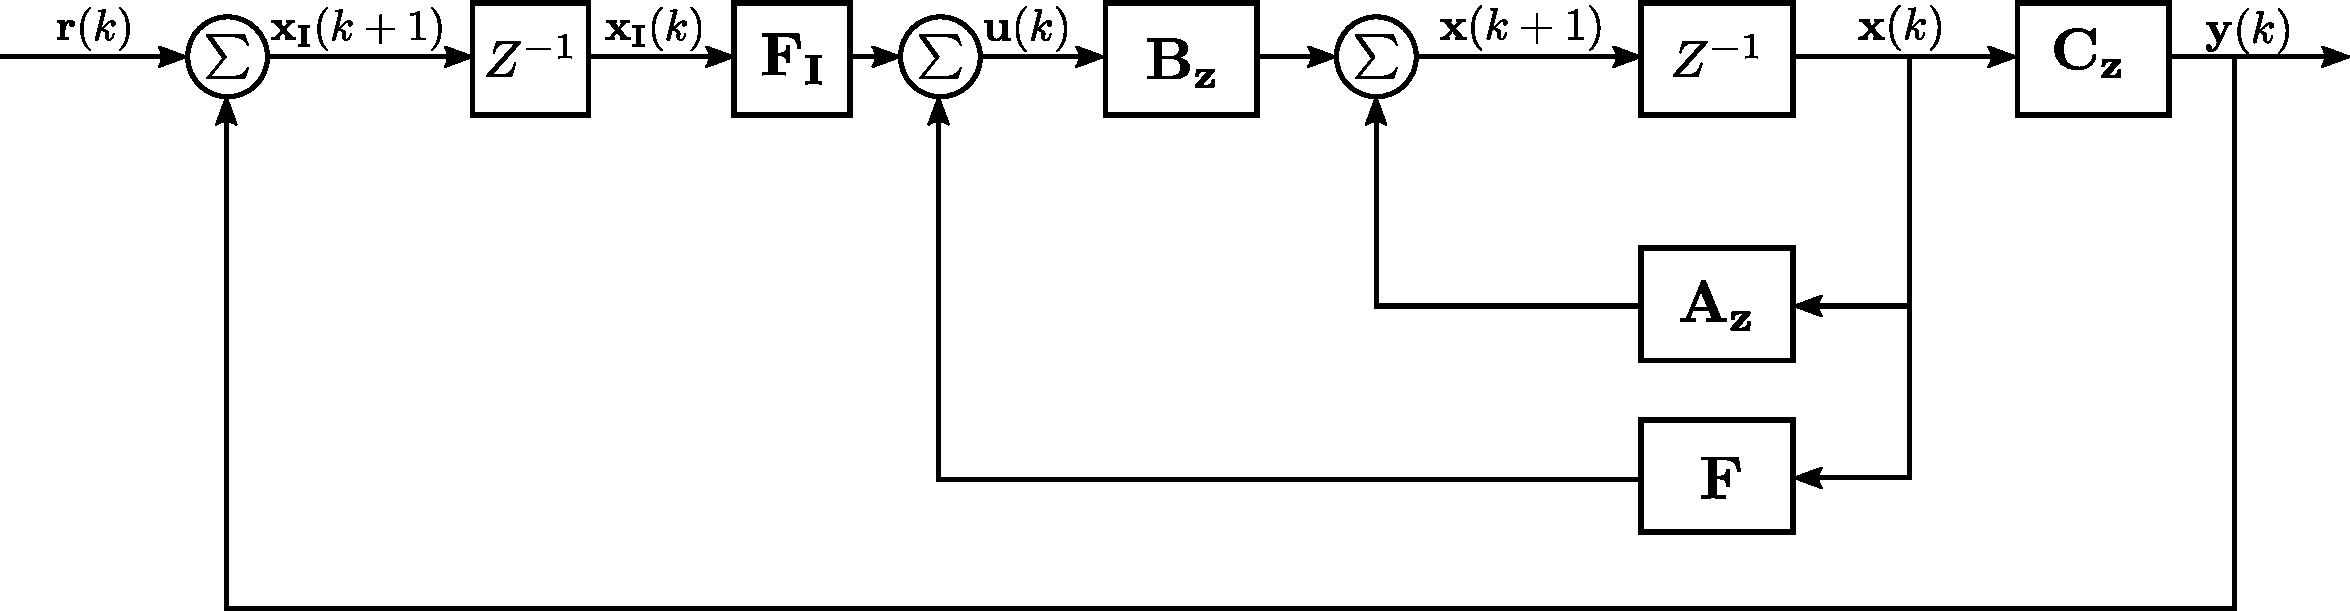
\includegraphics[width=0.9\textwidth]{figures/integralControlBlockDiagram}
  \caption{Block diagram of the control structure in the discrete domain.}
  \label{fig:blockConrolDesignLQR}
\end{figure}
%
To design this feedback system, it is convenient to express it on the following form:
\begin{flalign}
  \vec{x_e}(k+1) &= \vec{A_e} \vec{x}(k) + \vec{B_e} \vec{u}(k) + \vec{r}(k)
  \label{eq:xDotLinearDiscrete} \\
  \vec{y}(k)     &= \vec{C_e} \vec{x}(k)  \ \ .
  \label{eq:yLinearDiscrete} 
\end{flalign}
%
To describe the control design in this form, the $\vec{A_e}$, $\vec{B_e}$ and $\vec{C_e}$ matrices must be constructed. From \autoref{fig:blockConrolDesignLQR}, the discrete state space model for the integral is derived and shown in \autoref{eq:xIDiscrete}.
%
\begin{flalign}
  \vec{x_I}(k+1) &= \vec{x_I}(k) + \vec{y}(k) + \vec{r}(k) \label{eq:xIDiscrete1}  \\
  \vec{x_I}(k+1) &= \vec{x_I}(k) - C_z \vec{x}(k) + \vec{r}(k)  \ \ .
  \label{eq:xIDiscrete}
\end{flalign}
%
This leads to the discrete state space model extended with the integral states expressed as
%
\begin{flalign}
  \begin{bmatrix}
    \vec{x}(k+1)  \\
    \vec{x_I}(k+1)
  \end{bmatrix}
  =
  \begin{bmatrix}
    \vec{A}_{\vec{z}_{3x3}} & \vec{O}_{_{3x2}} \\
   -\vec{C}_{\vec{z}_{2x3}} & \vec{I}_{_{2x2}} \\
  \end{bmatrix}
  \begin{bmatrix}
    \vec{x}(k)    \\
    \vec{x_I}(k)
  \end{bmatrix}
  +
  \begin{bmatrix}
    \vec{B}_{\vec{z}_{3x2}} \\
    \vec{O}_{2x2}
  \end{bmatrix}
  \vec{u}(k)
  +
  \begin{bmatrix}
    \vec{O}_{3x2} \\
    \vec{I}_{2x2}
  \end{bmatrix}
  \vec{r}(k)
  \label{eq:discreteSSWithIntegralX}
\end{flalign}  
%
\begin{flalign}
  \vec{y}(k)
  =
  \begin{bmatrix}
    \vec{C}_{\vec{z}_{2x3}} &  \vec{O}_{2x2}
  \end{bmatrix}
  \begin{bmatrix}
    \vec{x}(k)    \\
    \vec{x_I}(k)
  \end{bmatrix}  \ \ ,
  \label{eq:discreteSSWithIntegralY}
\end{flalign}  
%
which corresponds to \autoref{eq:xDotLinearDiscrete} and \ref{eq:yLinearDiscrete}.

A discrete time infinite horizon LQR is used in the design of the feedback, $\vec{F_e} = [\ \vec{F} \ \ \vec{F}_\mathrm{I} ]\ $, which works by minimizing the cost function,
%
\begin{flalign}
  J = \sum_{k=0}^\infty \vec{x}_k^\mathrm{T}\vec{Q_d}\vec{x}_k + \vec{u}_k^\mathrm{T}\vec{R_d}\vec{u}_k  \ \ .
\end{flalign}
\begin{where}
	\va{\vec{Q_d}}{is the discrete time symmetric positive semidefinite state cost matrix}{}
  \va{\vec{R_d}}{is the discrete time symmetric positive definite input cost matrix}{}
\end{where}

The $\vec{Q_d}$ matrix contains the penalties for the states, such that a higher cost is generated for more critical states, thus driving these states faster to zero. The $\vec{R_d}$ matrix contains the penalties for the inputs. This helps to ensure the inputs are not driven towards saturation.

It is necessary for all states to be stable and controllable. Otherwise the the performance index, $J$, will become infinite \cite[p. 125]{DSNaidu}.\\
The controllability is determined by
%
\begin{flalign}
  \vec{{\mathcal C}}
  = 
  \begin{bmatrix}
    \vec{B}_\mathrm{e} & \vec{A}_\mathrm{e}\vec{B}_\mathrm{e} & \vec{A}_\mathrm{e}^{2} \vec{B}_\mathrm{e} & \vec{A}^{3}_\mathrm{e} \vec{B}_\mathrm{e} & \vec{A}^{4}_\mathrm{e} \vec{B}_\mathrm{e}
  \end{bmatrix}  \ \ ,
  \label{eq:integralControllability}
\end{flalign}
%
of which the rank is 5, that is, the controllability matrix, $\vec{{\mathcal C}}$, has full rank, thus the system is controllable \cite[p. 169]{CTChen}.\\
The eigenvalues of $\vec{A}_\mathrm{e}$ are all on or within the unit-circle in the z-plane, thus, no states are unstable and the LQR design is feasible.

The design approach taken to describe the cost function, $J$, is done by defining weights on the states and inputs for the continuous time infinite horizon LQR cost function,
%
\begin{flalign}
  J_{cont} = \int_{0}^\infty \vec{x}_k^\mathrm{T}\vec{Q}\vec{x}_k + \vec{u}_k^\mathrm{T}\vec{R}\vec{u}_k \  dt\ \ .
  \label{eq:contLQRcost}
\end{flalign}
\begin{where}
  \va{\vec{Q}}{is the continuous time symmetric positive semidefinite state cost matrix}{}
  \va{\vec{R}}{is the continuous time symmetric positive definite input cost matrix}{}
\end{where}

Bryson's rule is used as an initial design method to determine sensible values for the state and input penalties of the $\vec{Q}$ and $\vec{R}$ matrices, as described in \autoref{eq:QRBryson}\\
%
\begin{flalign} 
  Q_{ii} &= \frac{1}{x_{i_\mathrm{max}}\text{}^2} \rule{30px}{0px} R_{ii} = \frac{1}{u_{i_\mathrm{max}} \text{}^2}
  \label{eq:QRBryson}
\end{flalign}
\begin{where}
  \va{x_{i_\mathrm{max}}}{are the maximum acceptable state values}{}
  \va{u_{i_\mathrm{max}}}{are the maximum acceptable input values}{}
\end{where}

The requirements stated in \autoref{sec:requirements} must be taken into account when determining the values of $x_{i_\mathrm{max}}$ and $u_{i_\mathrm{max}}$. As the USV needs a high accuracy for bathymetric measurements, the weights of $\vec{Q}$ are set higher than $\vec{R}$ to ensure priority is focused on driving the states down to zero. The individual integral states are penalized higher than the system states to set further importance on driving the integral states to zero. This will ensure the reference signals are closely tracked. The low weights for $\vec{R}$ also ensures the actuators are not overexerted. This means the actuators will not be driven to saturation and will be used less. This is also ideal for the mobile vessel as the actuators will use less energy, thus the USV will be able to perform longer surveys.

These $\vec{Q}$ and $\vec{R}$ matrices must be discretized, as the state feedback design is done in the discrete time domain. \\
With
%
\begin{flalign}
  \vec{\Phi}(\tau) = e^{\vec{A}\tau} \\
  \vec{\Gamma}(\tau) = \int_{0}^{\tau}e^{\vec{A}\eta}\vec{B}d\eta
\end{flalign}
%
the weighting matrices, $\vec{Q}$ and $\vec{R}$, are discretized using \cite{lqrd}
\begin{flalign}
  \begin{bmatrix}
    \vec{Q_d} & 0 \\
    0 & \vec{R_d} 
  \end{bmatrix}
  = \int_{0}^{T_s}
  \begin{bmatrix}
    \vec{\Phi}^T(\tau)      & 0 \\
    \vec{\Gamma}^T(\tau)    & I
  \end{bmatrix}
  \begin{bmatrix}
    \vec{Q} & 0 \\
    0 & \vec{R}
  \end{bmatrix}
  \begin{bmatrix}
    \vec{\Phi}(\tau)  &   \vec{\Gamma}(\tau) \\
    0           &   I
  \end{bmatrix}
  d\tau
\end{flalign}
%The chosen values for Q and R are shown in \autoref{eq:QRMatrices}.
%
% 
% \begin{flalign}
%   \vec{Q} = 
%   \begin{bmatrix}
%     100 & 0   & 0   & 0   & 0             \\
%     0   & 100 & 0   & 0   & 0             \\
%     0   & 0   & 100 & 0   & 0             \\
%     0   & 0   & 0   & 400 & 0             \\
%     0   & 0   & 0   & 0   & 400
%   \end{bmatrix} \rule{30px}{0px}
%   \vec{R} = 
%   \begin{bmatrix}
%     25\times10^{-6}   & 0                 \\
%     0                 & 25\times10^{-6}
%   \end{bmatrix}
%   \label{eq:QRMatrices}
% \end{flalign}
%
From this the state feedback is calculated by \cite[p. 42]{JLNy},
%
\begin{flalign}
  \vec{F}_\mathrm{e} &= -(\vec{B}_\mathrm{e}^\mathrm{T} \vec{P}\vec{B}_\mathrm{e} + \vec{R_d})^{-1}  \vec{B}_\mathrm{e}^\mathrm{T} \vec{P}\vec{A}_\mathrm{e} \ \ ,
  \label{eq:QRFeedback}
\end{flalign}
%
where $\vec{P}$ can be found as the solution of the infinite horizon algebraic discrete-time Riccati equation \cite[p. 42]{JLNy},
%
\begin{flalign}
\vec{P} &= \vec{A}_\mathrm{e}^\mathrm{T} \vec{P} \vec{A}_\mathrm{e} + \vec{Q_d} - \vec{A}_\mathrm{e}^\mathrm{T} \vec{P} \vec{B}_\mathrm{e} (\vec{B}_\mathrm{e}^\mathrm{T} \vec{P} \vec{B}_\mathrm{e} + \vec{R_d})^{-1} \vec{B}_\mathrm{e}^\mathrm{T} \vec{P} \vec{A}_\mathrm{e} \ \ .
\label{eq:discreteInfRiccati}
\end{flalign}
%
Once $\vec{F}_\mathrm{e}$ is obtained, it is split into the two feedback matrices, $\vec{F}_\mathrm{e} = [\ \vec{F} \ \ \vec{F}_\mathrm{I}\ ]$, and implemented, following the control structure provided in \autoref{fig:blockConrolDesignLQR}.

These design has been simulated together with the nonlinear model of the system. Its performance is also compared to the $\mathcal{H}_\infty$ controller designed in \autoref{sec:Hinf} when disturbances, measurement noise and parameter uncertainties are present. The simulations are presented in \autoref{sec:comparison}.









